% !TEX encoding = UTF-8
% !TEX program = lualatex

\documentclass[a4paper]{article}

\usepackage[left=1.5cm, right=1.5cm, top=1cm, bottom=2cm]{geometry}

\usepackage{mathtools, amssymb}
    \def\RR{\mathbf R}
    \def\CC{\mathbf C}

\usepackage[no-math]{fontspec}
    \setmainfont{Noto Serif}
    \setsansfont{Noto Sans TC}
    \setmonofont{Noto Sans Mono}

\usepackage{tikz}

\begin{document}

\parindent 0pt
\parskip 1em

\newcounter{p}
\def\Problem{\stepcounter{p}[\thep] }
\newcounter{c}
\def\yes{\no}
\def\no{\hskip0pt plus1em\stepcounter c%
    \ifnum\value c=27\setcounter c1\fi(\Alph c) }
    
\section*{Complex Variable - Midterm Mock Exam}

\sffamily

考試時間 Test time 10:30:00 am to 12:00:00 pm; 1.5 hours.
以教室投影機時鐘為準 Using the projected clock.
用空白紙張作答 Answer on blank paper.
每個問號一分 One point per question mark.
全對才給分 No partial credit.
可以帶 991 You can use fx-991 or anything weaker.
舉手問問題 Raise your hand to ask questions.

\rmfamily

\Problem
A vector is ?-free if $P_x + Q_y = 0$.
Which of the following picture is this-free?

\no \raisebox{-2cm}{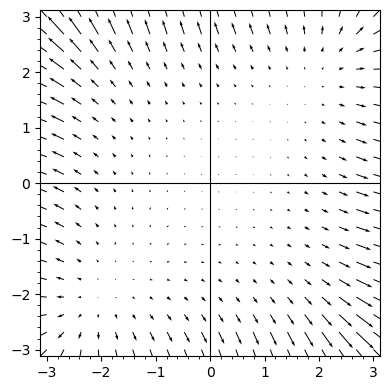
\includegraphics[width=4cm]{div.png}}
\yes \raisebox{-2cm}{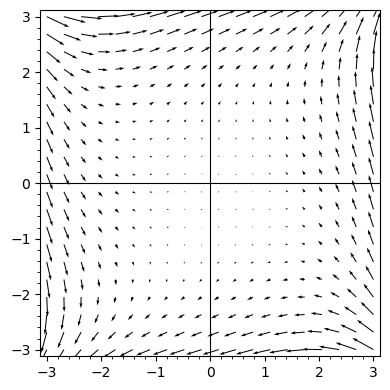
\includegraphics[width=4cm]{curl.png}}

\Problem
A vector is ?-free if $P_y = Q_x$.
Which of the picture above is this-free?

\Problem
Select all that apply.
For $u\colon \RR^2 \to \RR$ a harmonic function,
The vector field $(u_x, u_y)$ is
\yes divergence-free
\yes curl-free
\no path dependent
\no diffeomorphic?

\Problem
Consider using the anti-derivative of $P - Qi$
to solve for fluid dynamics problems.
Which are correct?
\yes fluid flows faster when the $\Psi$ contours are closer.
\yes fluid flows faster when the $\Phi$ contours are closer.
\no fluid flows faster when the $\Psi$ contours are farther.
\no fluid flows faster when the $\Phi$ contours are farther.

\Problem
What condition is not needed when proving that
a subset of $\CC$ is $\CC$ itself?
\no nonempty
\no open
\no close
\no compact

\Problem
The lower left picture is the domain coloring plot of $h(z) = z$.
The lower picture is $?(? - z) / (z + ?)$.
(All question marks are Gaussian integers.)

\raisebox{-2cm}{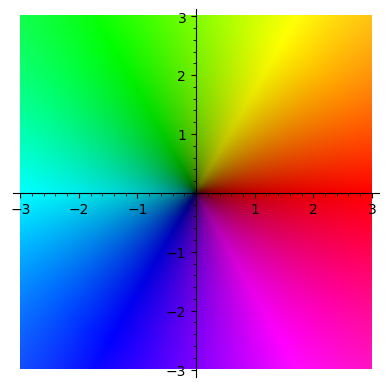
\includegraphics[width=4cm]{z.png}}
\raisebox{-2cm}{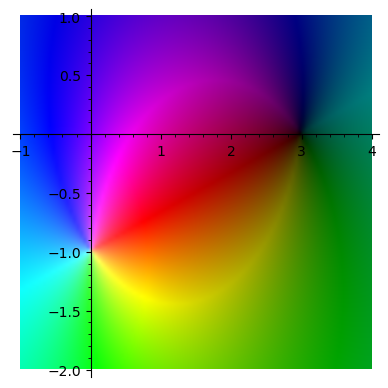
\includegraphics[width=4cm]{mo.png}}

\Problem
Decompose the Mobius map $d (z - a) / (z - b)$
into to a composition of $+c$, $c\cdot$, and $^{-1}$.
\[
    \CC \longrightarrow \CC \longrightarrow \CC \longrightarrow
    \CC \longrightarrow \CC \longrightarrow \CC \longrightarrow
    \CC \longrightarrow \CC \longrightarrow \CC \longrightarrow
    \CC \longrightarrow \CC \longrightarrow \CC \longrightarrow
    \CC \longrightarrow \CC \longrightarrow \CC \longrightarrow
    \CC
\]

\Problem
Consider the Mobius map $g(z) = 6 / (7 - z)$.
Let $G$ be the composition of $10$ $g$'s,
then $1 / G'(1) = 60466???$.

\Problem
The conformal map $z \mapsto z + 1/z$ maps what
to the upper half plane?
Draw on the canvas.

\raisebox{-2cm}{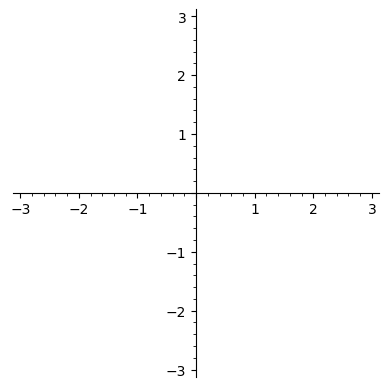
\includegraphics[width=4cm]{white.png}}

\Problem
$\exp(2000 + i) = ?.??70106084616010^{868} + ?.??59005203013710^{868} i$.

\Problem
Define a complex $\ln$ function such that $\ln(1) = 0$
and is continuous at points not on the spiral.
What is $\ln(3 + 3i)$???

\raisebox{-2cm}{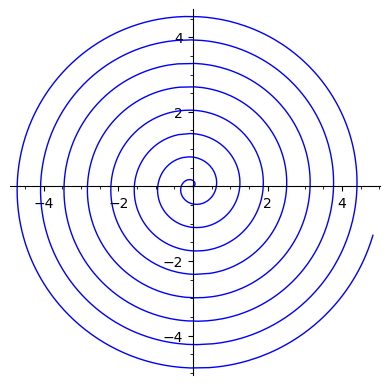
\includegraphics[width=4cm]{spiral.png}}

\Problem
Let $f$ be an arbitrary holomorphic function.
The integral $\int_0^\infty \frac{f(x^3)}{1 + x^3}dx$
can be expressed using $f$ as ???
(Do not use the integral symbol in your answer.)

\Problem
Consider an integral of the form $\int_{-1}^2 f(x) \, dx$.
If $f$ is meormorphic and has a pole at $x = 0$,
then it probably does not converge.
Its (Cauchy) principal value is defined as
$\lim_{\delta\to0} \int_{?}^{?} f(x) \, dx + \int_{?}^{?} f(x) \, dx$.
For $h(x) = \sin(x) / x^4$, the principal value is $0.0???841052008818$.

\Problem
The Schwarz--Christoffel formula
$f(\zeta) = \int_0^\zeta (z + 1)^{-?} (z + 2)^{-?} \, dz$
maps the upper half plane to a equilateral triangle.
The number ? is mapped to the lower left corner.
The number ? is mapped to the lower right corner.
The number ? is mapped to the top corner.
The side length is $?.2999162508563$.

\Problem
List three (???) bijective conformal maps from the upper half plane
to the triangle in the previous problem,
and they must be different from the $f$ above.
If there are not enough functions, write down NOMORE.

\Problem
For a harmonic function $u\colon \CC \to \RR$,
there exists another harmonic function $v\colon \CC \to \RR$
such that $u + iv$ is holomorphic.
Let $u(x, y) = -(y^2 - x^2 - 1)/(4 y^2 x^2 + (y^2 - x^2 - 1)^2)$
and $v(0, 0) = 0$.
Then $v(1, 1.5) = -0.???034482758621$.

\Problem
Consider the Dirichlet problem on a circle.
That is, $u$ is harmonic inside the circle,
continuously extending to the boundary,
and $u(e^{i\theta}) = \beta(\theta)$
for the boundary condition $\beta(\theta) = \cos(\theta)^{72}$.
Then $u(0 + 0i) = 0.???770122224943$.

\Problem
If $f$ and $g$ are holomorphic functions on the entire $\CC$
and $f(1/n) = g(1/n)$ for all positive integer $n$,
why is $f = g$ on the entire $\CC$?
(Tell me the name of the theorem used.)
If $f$ and $g$ are holomorphic on the punctured plane $\CC \setminus \{0\}$,
does $f = g$ still hold or you can find a counterexample???

\end{document}